%%%%%%%%%%%%%%%%%%%%%%%%%%%%%%%%%%%%%%%%%%%%%%%%%%%%%%%%%%%%%%%%%%%%%%%%%%%%
%% Header

\documentclass[20pt]{beamer}

\usepackage[utf8]{inputenc}
\usepackage[english]{babel}
\usepackage{beamerthemesplit}
\usepackage{listings}
\usepackage{graphicx}
\usepackage{colortbl}
\usepackage{floatflt}
\usepackage{wasysym}
\usepackage{lmodern}
\usepackage{tikz}

\title{Toward Monad Transformers}
\author{Antoine Leblanc - @nicuveo}
\institute{Functional Programmers Paris}
\date{\small{2015-04-01}}



%%%%%%%%%%%%%%%%%%%%%%%%%%%%%%%%%%%%%%%%%%%%%%%%%%%%%%%%%%%%%%%%%%%%%%%%%%%%
%% Customization

%%%%%%%%%%%%%%%%%%%%%%%%%%%%%%%%%%%%%%%%%%%%%%%%%%%%%%%%%%%%%%%%%%%%%%%%%%%%
%% Base theme

\mode<presentation>{}
\usecolortheme{whale}
\usepackage{fontspec}
\usepackage{etoolbox}
\setmonofont{Ubuntu Mono}
\setsansfont[Ligatures=TeX, ItalicFont={* Italic}]{League Gothic}



%%%%%%%%%%%%%%%%%%%%%%%%%%%%%%%%%%%%%%%%%%%%%%%%%%%%%%%%%%%%%%%%%%%%%%%%%%%%
%% Colors

% define

\definecolor{my-color-1}{RGB}{204,   0,   0} % primary
\definecolor{my-color-2}{RGB}{ 51,  51, 151} % lighter
\definecolor{my-color-3}{RGB}{  0,   0,   0} % unknown
\definecolor{my-color-4}{RGB}{  0,   0,   0} % darker

\definecolor{tab-1}{rgb}{0.04,0.34,0.58}
\definecolor{tab-2}{rgb}{0.36,0.56,0.72}
\definecolor{tab-3}{rgb}{0.68,0.78,0.86}


% set

\setbeamercolor{structure}{fg=my-color-1}
\setbeamercolor{alerted text}{fg=my-color-1!56!red}

\setbeamercolor{palette primary}   {fg=white, bg=my-color-1}
\setbeamercolor{palette secondary} {fg=black, bg=my-color-2}
\setbeamercolor{palette tertiary}  {fg=white, bg=my-color-3}
\setbeamercolor{palette quaternary}{fg=white, bg=my-color-4}

\setbeamercolor{page number in head/foot} {fg=black, bg=white}
\setbeamercolor{icon in head/foot} {fg=black, bg=white}

\setbeamercolor*{separation line}{}
\setbeamercolor*{fine separation line}{}



%%%%%%%%%%%%%%%%%%%%%%%%%%%%%%%%%%%%%%%%%%%%%%%%%%%%%%%%%%%%%%%%%%%%%%%%%%%%
%% Templates

\AtBeginSection[]
{
  \begin{frame}
    \hypersetup{hidelinks}
    \frametitle{Outline}
    \tableofcontents[currentsection,hideothersubsections]
  \end{frame}
}

\setbeamertemplate{section in toc shaded}{\hspace*{1em}\color{white}$\blacktriangleright$\color{black}~~\inserttocsection}
\setbeamertemplate{section in toc}{\hspace*{1em}$\blacktriangleright$~~\inserttocsection!}

\makeatletter
\Hy@AtBeginDocument{%
  \def\@pdfborder{0 0 1}% Overrides border definition set with colorlinks=true
  \def\@pdfborderstyle{/S/U/W 1}% Overrides border style set with colorlinks=true
                                % Hyperlink border style will be underline of width 1pt
}
\patchcmd{\beamer@sectionintoc}{\vskip1.5em}{\vskip0.5em}{}{}
\makeatother

\hypersetup{%
  colorlinks=true,
  urlcolor=my-color-2,
  urlbordercolor=my-color-2
}

\newtoggle{showpagenumber}

\setbeamertemplate{headline}[default]

\defbeamertemplate{footline}{mine}[2]
{
  \leavevmode%
  \hbox
  {%
    \ifstrempty{#1}{%
    \hskip .180\paperwidth%
    }{%
    \hskip .020\paperwidth
    \begin{beamercolorbox}[wd=.160\paperwidth,ht=3ex,dp=3ex,center]{icon in head/foot}
      \usebeamerfont{page number in head/foot}
      \pgfimage[mask=#2,interpolate=true,height=20pt]{#1}
    \end{beamercolorbox}%
    }%

    \hskip .720\paperwidth

    \begin{beamercolorbox}[wd=.100\paperwidth,ht=3ex,dp=3ex,center]{page number in head/foot}
      \usebeamerfont{page number in head/foot}
      \iftoggle{showpagenumber}{
        \insertframenumber{} / \inserttotalframenumber{}
      }{}
      \end{beamercolorbox}%
  }%
  \vskip0pt%
}

\newcommand{\setfooterlogo}[2]
{
  \setbeamertemplate{footline}[mine]{#1}{#2}
}

%\pgfdeclaremask{masklogo}{img/logo}
\newcommand\defaultlogo{\setfooterlogo{}{}}
\defaultlogo

\setbeamersize{text margin left=10pt,text margin right=10pt}



%%%%%%%%%%%%%%%%%%%%%%%%%%%%%%%%%%%%%%%%%%%%%%%%%%%%%%%%%%%%%%%%%%%%%%%%%%%%
%% Code environnement

\definecolor{hsk-comment} {gray}{0.6}
\colorlet{hsk-built-ins}{my-color-3!50!blue}
\colorlet{hsk-types} {my-color-1}
\colorlet{hsk-operators}{my-color-1!50!black}
\colorlet{hsk-keywords} {my-color-1!50!black}
\colorlet{hsk-consts} {my-color-1!50!blue}
\colorlet{hsk-string} {my-color-1!50!red}

\lstdefinelanguage{ColorHaskell} {
        basicstyle=\ttfamily\footnotesize,
        sensitive=true,
        morecomment=[l][\color{hsk-comment}\ttfamily\itshape]{--},
        morecomment=[s][\color{hsk-comment}\ttfamily\itshape]{\{-}{-\}},
        morestring=[b]",
        stringstyle=\color{hsk-string},
        showstringspaces=false,
%        numberstyle=\footnotesize
        showspaces=false,
        breaklines=true,
        showtabs=false,
        emph=
        {[1]
                abs,acos,acosh,all,and,any,appendFile,approxRational,asTypeOf,asin,
                asinh,atan,atan2,atanh,basicIORun,break,catch,ceiling,chr,compare,concat,concatMap,
                const,cos,cosh,curry,cycle,decodeFloat,denominator,digitToInt,divMod,drop,
                dropWhile,either,encodeFloat,enumFrom,enumFromThen,enumFromThenTo,enumFromTo,
                error,even,exp,exponent,fail,filter,flip,floatDigits,floatRadix,floatRange,floor,
                fmap,foldl,foldl1,foldr,foldr1,fromDouble,fromEnum,fromInt,fromInteger,fromIntegral,
                fromRational,fst,gcd,getChar,getContents,getLine,head,id,inRange,index,init,intToDigit,
                interact,ioError,isAlpha,isAlphaNum,isAscii,isControl,isDenormalized,isDigit,isHexDigit,
                isIEEE,isInfinite,isLower,isNaN,isNegativeZero,isOctDigit,isPrint,isSpace,isUpper,iterate,
                last,lcm,length,lex,lexDigits,lexLitChar,lines,log,logBase,lookup,map,mapM,mapM_,max,
                maxBound,maximum,maybe,min,minBound,minimum,negate,not,null,numerator,odd,
                or,ord,otherwise,pi,pred,primExitWith,print,product,properFraction,putChar,putStr,putStrLn,
                quotRem,range,rangeSize,read,readDec,readFile,readFloat,readHex,readIO,readInt,readList,readLitChar,
                readLn,readOct,readParen,readSigned,reads,readsPrec,realToFrac,recip,repeat,replicate,return,
                reverse,round,scaleFloat,scanl,scanl1,scanr,scanr1,sequence,sequence_,show,showChar,showInt,
                showList,showLitChar,showParen,showSigned,showString,shows,showsPrec,significand,signum,sin,
                sinh,snd,span,splitAt,sqrt,subtract,succ,sum,tail,take,takeWhile,tan,tanh,threadToIOResult,toEnum,
                toInt,toInteger,toLower,toRational,toUpper,truncate,uncurry,undefined,unlines,until,unwords,unzip,
                unzip3,userError,words,writeFile,zip,zip3,zipWith,zipWith3,listArray,doParse
        },
        emphstyle={[1]\color{hsk-built-ins}},
        emph=
        {[2]
                FilePath,IOError,Bool,Char,Double,Either,Float,IO,Integer,Int,Maybe,Ordering,Rational,Ratio,ReadS,ShowS,String, Word8,InPacket
        },
        emphstyle={[2]\color{hsk-types}},
        emph=
        {[3]
                case,class,data,deriving,do,else,if,import,in,infixl,infixr,instance,let,
                module,of,primitive,then,type,where
        },
        emphstyle={[3]\color{hsk-keywords}\textbf},
        emph=
        {[4]
                quot,rem,div,mod,elem,notElem,seq
        },
        emphstyle={[4]\color{hsk-operators}\textbf},
        emph=
        {[5]
                EQ,False,GT,Just,LT,Left,Nothing,Right,True,Show,Eq,Ord,Num,Enum,Bounded
        },
        emphstyle={[5]\color{hsk-consts}\textbf},
        flexiblecolumns=false,
        mathescape=false,
        basewidth={0.5em,0.45em},
        literate={+}{{$+$}}1
                 {/}{{$/$}}1
                 {*}{{$*$}}1
                 {=}{{$=$}}1
                 {>}{{$>$}}1
                 {<}{{$<$}}1
                 {\\}{{$\lambda$}}1
                 {->}{{$\rightarrow$}}2
                 {>=}{{$\geq$}}2
                 {<-}{{$\leftarrow$}}2
                 {<=}{{$\leq$}}2
                 {=>}{{$\Rightarrow$}}2
                 {>>}{{>>}}2
                 {>>=}{{>>=}}3
                 {>=>}{{>=>}}3
                 {|}{{$\mid$}}1
}

\lstnewenvironment{code}{\lstset{language=ColorHaskell}}{}
\lstnewenvironment{smallCode}{\lstset{language=ColorHaskell,basicstyle=\tiny\ttfamily}}{}
\newcommand{\inline}[1]
{
  {\lstinline[language=ColorHaskell]|#1|}
}



%%%%%%%%%%%%%%%%%%%%%%%%%%%%%%%%%%%%%%%%%%%%%%%%%%%%%%%%%%%%%%%%%%%%%%%%%%%%
%% Fonts

\setbeamerfont{frametitle}{size=\small}
\setbeamerfont{structure}{series=\bfseries}



%%%%%%%%%%%%%%%%%%%%%%%%%%%%%%%%%%%%%%%%%%%%%%%%%%%%%%%%%%%%%%%%%%%%%%%%%%%%
%% Settings

\setbeamertemplate{navigation symbols}{}

\bibliographystyle{apalike}

\mode<all>


\renewcommand{\(}[1]{\begin{columns}[#1]}
\renewcommand{\)}{\end{columns}}
\newcommand{\<}[1]{\begin{column}{#1\textwidth}}
\renewcommand{\>}{\end{column}}



%%%%%%%%%%%%%%%%%%%%%%%%%%%%%%%%%%%%%%%%%%%%%%%%%%%%%%%%%%%%%%%%%%%%%%%%%%%%
%% Document

\begin{document}



%% Joke frame

%\togglefalse{showpagenumber}
%\begin{frame}
%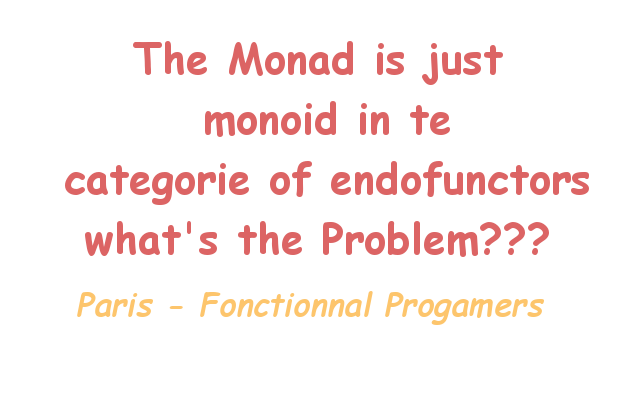
\includegraphics[width=\paperwidth]{img/joke}
%\end{frame}
%\begin{frame}
%
\includegraphics[width=\paperwidth]{img/fish}
%\end{frame}



%% Title frame

{

\usebackgroundtemplate{%
\vbox to \paperheight{\vfil\hbox to \paperwidth{\hfil
\includegraphics[width=8cm]{img/title}\hfil}\vfil}
}
\togglefalse{showpagenumber}
\begin{frame}[fragile]
  \titlepage
\end{frame}

}

\toggletrue{showpagenumber}
\setcounter{framenumber}{0}



%% Monads

\section{Monads}

\begin{frame}
\frametitle{Introduction}
\href{http://www.stephendiehl.com/what/}{What I Wish I Knew When Learning Haskell}
\pause
~\\~\\
\begin{quote}
    1. Don't read the monad tutorials.\\\pause
    2. No really, don't read the monad tutorials.\\\pause
    ~~~~~\ldots\\\pause
    8. Don't write monad-analogy tutorials.
\end{quote}
\end{frame}

\begin{frame}[fragile]
  \frametitle{Typeclass}
  \begin{code}
    class Monad m where
        return :: a -> m a
        (>>=)  :: m a -> (a -> m b) -> m b
  \end{code}
  \begin{overlayarea}{\paperwidth}{4cm}
    \begin{onlyenv}<2>
    \begin{center}
    \vspace{0.2cm}
    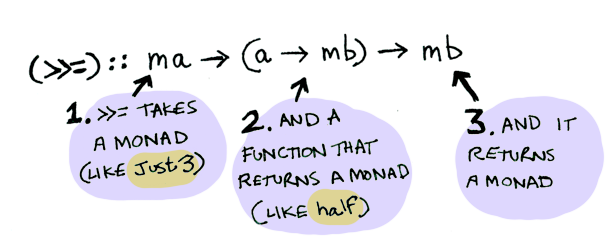
\includegraphics[height=3cm]{img/monad} \\
    \href{http://adit.io/posts/2013-04-17-functors,_applicatives,_and_monads_in_pictures.html}{\tiny adit.io}
    \end{center}
    \end{onlyenv}
    \begin{onlyenv}<3>
    \begin{code}
    (>>)  :: Monad m => m a -> m b -> m b
    (>=>) :: Monad m => (a -> m b)
                     -> (b -> m c)
                     -> (a -> m c)
    \end{code}
    \end{onlyenv}
  \end{overlayarea}
\end{frame}

\begin{frame}[fragile]
  \frametitle{Monad laws}
  Using \alt<1>{\inline{(>>=)}}{\inline{(>=>)}}\\

  \begin{center}
    \only<1>
    {
      \begin{tabular}{ r c l }
        \inline{return a >>= f}  & $~\equiv~$ & \inline{f a} \\
        \inline{m >>= return}    & $~\equiv~$ & \inline{m}   \\
        \inline{(m >>= f) >>= g} & $~\equiv~$ & \inline{m >>= (\\x -> f x >>= g) }
      \end{tabular}
    }
    \only<2>
    {
      \begin{tabular}{ r c l }
        \inline{return >=> f}    & $~\equiv~$ & \inline{f} \\
        \inline{f >=> return}    & $~\equiv~$ & \inline{f} \\
        \inline{(f >=> g) >=> h} & $~\equiv~$ & \inline{f >=> (g >=> h) }
      \end{tabular}
    }
  \end{center}
\end{frame}

\begin{frame}[fragile]
  \frametitle{Do notation}
  \begin{center}
    \begin{tabular}{ r c l }
      \inline{do \{ a <- f ; m \}} & $~\equiv~$ & \inline{f >>= \\a -> m} \\
      \inline{do \{ f ; m \}}      & $~\equiv~$ & \inline{f >> m}         \\
      \inline{do \{ m \}}          & $~\equiv~$ & \inline{m}
    \end{tabular}
  \end{center}
\end{frame}

\begin{frame}[fragile]
  \frametitle{Do sugar}
  \({b}
  \<{0.5}
  \begin{code}
 f >>= \a ->
   g >>= \b ->
     h >>= \c ->
       return (a, b, c)
  \end{code}
  \>
  \pause
  \<{0.5}
  \begin{code}
 do
     a <- f
     b <- g
     c <- h
     return (a, b, c)
  \end{code}
  \>
  \)
\end{frame}

\begin{frame}
  \frametitle{ALL TEH MONADS}
  \vspace{-1cm}
  \begin{center}
    \begin{tabular}{ l l }
      \uncover<1->{\\ Maybe    & \inline{getUser :: Id -> Maybe User}}
      \uncover<2->{\\ Either a & \inline{parse :: String -> Either Error Value}}
      \uncover<3->{\\ List     & \inline{allNextTurns :: Board -> [Board]}}
      \uncover<4->{\\ IO       & \inline{httpGet :: Url -> IO String}}
      \uncover<5->{\\ Reader r & \inline{runReader :: Reader r a -> r -> a}}
      \uncover<6->{\\ Writer w & \inline{runWriter :: Writer w a -> (a, w)}}
      \uncover<7->{\\ State s  & \inline{runState  :: Reader s a -> s -> (a, s)}}
    \end{tabular}
    \uncover<7->{
\includegraphics[height=2cm]{img/all}}
  \end{center}
\end{frame}

\newcommand{\BSQR}[1]{{\color{#1}\blacksquare}}
\newcommand{\FUNC}[2]{(#1 \rightarrow #2)}
\newcommand{\READ}[1]{\boxed{\BSQR{red} \rightarrow \BSQR{#1}}}
\newcommand{\WRIT}[1]{\boxed{\BSQR{#1}~~\BSQR{red}}}
\newcommand{\STAT}[1]{\boxed{\BSQR{red} \rightarrow \BSQR{#1}~~\BSQR{red}}}

\begin{frame}[fragile]
  \frametitle{Reader Monad}
  \begin{center}
    \begin{tabular}{ r c l }
 \inline{Reader Green}  & $::$ & $\READ{green}$ \\
 \inline{Reader Yellow} & $::$ & $\READ{yellow}$ \\
 &&\\
 \inline{(>>=)} & $::$ & $\READ{green}$ \\
       & $\rightarrow$ & $\FUNC{\BSQR{green}}{\READ{yellow}}$ \\
       & $\rightarrow$ & $\READ{yellow}$ \\
 &&\\
 \inline{runReader} & $::$ & $\READ{yellow} \rightarrow \FUNC{\BSQR{red}}{\BSQR{yellow}}$ \\
    \end{tabular}
  \end{center}
\end{frame}

\begin{frame}[fragile]
  \frametitle{Reader example}
  \begin{center}
    \begin{code}
  data Conf = { color :: Color, size :: Int }

  formatter :: String -> Reader Conf String
  formatter p = do
      c <- asks color
      s <- asks size
      return (undefined) -- TODO

  format :: Conf -> String -> String
  format c s = runReader (textFormatter s) c
    \end{code}
  \end{center}
\end{frame}

\begin{frame}[fragile]
  \frametitle{Writer Monad}
  \begin{center}
    \begin{tabular}{ r c l }
 \inline{Writer Green}  & $::$ & $\WRIT{green}$ \\
 \inline{Writer Yellow} & $::$ & $\WRIT{yellow}$ \\
 &&\\
 \inline{(>>=)} & $::$ & $\WRIT{green}$ \\
       & $\rightarrow$ & $\FUNC{\BSQR{green}}{\WRIT{yellow}}$ \\
       & $\rightarrow$ & $\WRIT{yellow}$ \\
 &&\\
 \inline{runWriter} & $::$ & $\WRIT{yellow} \rightarrow (\BSQR{yellow}~~\BSQR{red})$ \\
    \end{tabular}
  \end{center}
\end{frame}

\begin{frame}[fragile]
  \frametitle{Writer example}
  \begin{center}
    \begin{code}
  type Log = [String]
  type Debug = Writer Log

  value :: Int -> Debug Int
  value x = Writer (x, ["Value"])

  plus :: Debug Int -> Debug Int -> Debug Int
  plus x y = do
      a <- x
      b <- y
      Writer (a + b, "Plus")
    \end{code}
  \end{center}
\end{frame}

\begin{frame}[fragile]
  \frametitle{State Monad}
  \begin{center}
    \vspace{-0.5em}
    \begin{tabular}{ r c l }
 \inline{State Green}  & $::$ & $\STAT{green}$ \\
 \inline{State Yellow} & $::$ & $\STAT{yellow}$ \\
 &&\\
 \inline{(>>=)} & $::$ & $\STAT{green}$ \\
       & $\rightarrow$ & $\FUNC{\BSQR{green}}{\STAT{yellow}}$ \\
       & $\rightarrow$ & $\STAT{yellow}$ \\
 &&\\
 \inline{runState} & $::$ & $\STAT{yellow}$ \\
            &$\rightarrow$& $\FUNC{\BSQR{red}}{\BSQR{yellow}~~\BSQR{red}}$ \\
    \end{tabular}
  \end{center}
\end{frame}

\begin{frame}[fragile]
  \frametitle{State Example}
  \begin{center}
    \begin{code}
  data GameInfo = GameInfo {
    turn :: Int,
    score :: Int
  }

  skipTurn :: State GameInfo ()
  skipTurn = do
      t <- gets turn
      s <- gets score
      put $ GameInfo (t + 1) (s `div` 2)
    \end{code} %$
  \end{center}
\end{frame}



%% Mission

\section{Our mission}

\begin{frame}
  \frametitle{REST client}
  \({b}
  \<{0.55}
  \begin{itemize}
    \item Authenticate
    \item Issue simple commands
    \item \emph{That's it!}
  \end{itemize}
  \vspace{2cm}
  \>
  \<{0.45}
  
\includegraphics[width=5cm]{img/rest}
  \>
  \)
\end{frame}

\begin{frame}[fragile]
  \frametitle{Monadic syntax?}
  \begin{code}
  main = run $ do
      setServerUrl   "http://server.com/api"
      setCredentials "guest" "guest"
      authenticate
      result <- request "server.listMyStuff"
      print $ format result
  \end{code}
\end{frame}

\begin{frame}[fragile]
  \frametitle{Problem}
  \begin{center}
    \begin{overlayarea}{\paperwidth}{2.4cm}
    \begin{onlyenv}<-3>
      \begin{code}
    import Network.HTTP.Conduit
    simpleHttp :: String -> IO ByteString
      \end{code}
      \vspace{0.8em}
    \end{onlyenv}
    \begin{onlyenv}<4->
      \begin{code}
    import Network.HTTP.Conduit
    simpleHttp :: MonadIO m =>
                  String -> m ByteString
      \end{code}
    \end{onlyenv}
    \end{overlayarea}
    ~\\
    \only<1>{~}
    \only<2>{\ttfamily{}IO!}
    \only<3>{\emph{wait\ldots{}}}
    \only<4>{\ldots{}\ttfamily{}MonadIO?}
  \end{center}
\end{frame}

\begin{frame}
  \frametitle{State in IO}
  \begin{itemize}
  \item MVar?
  \item IORef?
  \end{itemize}
  \pause
  \begin{center}
    ...add State and Either monads to IO?
  \end{center}
\end{frame}



%% Transformers

\section{Transformers}

\begin{frame}
  \frametitle{All the way down}
  \({b}
  \<{0.6}
  \begin{itemize}
    \item Monad generalization
    \item Extra monad parameter
    \item Monad stacks
  \end{itemize}
  \>
  \<{0.4}
  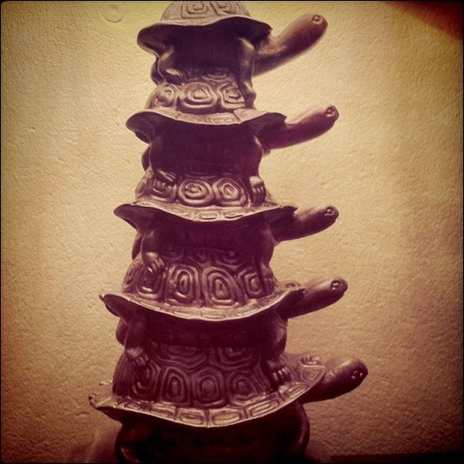
\includegraphics[width=3cm]{img/turtles}
  \>
  \)
\end{frame}

\begin{frame}[fragile]
  \frametitle{Monad $\rightarrow$ MonadT}
  \vspace{1cm}
  \begin{onlyenv}<1>
    \begin{code}
    data State s a = { ... }
    get :: State s s
    put :: s -> State s ()
    \end{code}
  \end{onlyenv}
  \begin{onlyenv}<2>
    \begin{code}
    data StateT s m a = { ... }
    get :: MonadState s m => m s
    put :: MonadState s m => s -> m ()
    \end{code}
  \end{onlyenv}
  \begin{center}
    \only<1>{
\includegraphics[height=3cm]{img/mr} \\\scriptsize Mister}
    \only<2>{
\includegraphics[height=3cm]{img/mrt}\\\scriptsize MisterT}
  \end{center}
\end{frame}

\begin{frame}[fragile]
  \frametitle{Lifting}
  \begin{onlyenv}<1>
    \begin{code}
    example :: CustomT IO Int
    example = do
        customStuff 1
        lift $ putStrLn "Turtles!"
        customStuff 2
    \end{code}%$
  \end{onlyenv}
  \begin{onlyenv}<2>
    \begin{code}
    example :: CustomT (MaybeT IO) Int
    example = do
        customStuff 1
        lift $ lift $ putStrLn "Turtles!"
        customStuff 2
    \end{code}%$
  \end{onlyenv}
\end{frame}

\begin{frame}[fragile]
  \frametitle{Instances}
  \begin{code}
    class Monad m => MonadState s m where
        get :: m s
        put :: s -> m ()

    instance MonadState s m =>
             MonadState s (ReaderT r m) where
        get = lift get
        put = lift . put
  \end{code}
\end{frame}

\begin{frame}[fragile]
  \frametitle{$n~^2$}
  \begin{center}
    \begin{tabular}{ l c l c l }
      \emph{IO} & $~\leftrightarrow~$ & MonadIO     & $~\leftrightarrow~$ & \inline{liftIO}     \\
      StateT    & $~\leftrightarrow~$ & MonadState  & $~\leftrightarrow~$ & \inline{get}        \\
      ReaderT   & $~\leftrightarrow~$ & MonadReader & $~\leftrightarrow~$ & \inline{ask}        \\
      WriterT   & $~\leftrightarrow~$ & MonadWriter & $~\leftrightarrow~$ & \inline{tell}       \\
      ErrorT    & $~\leftrightarrow~$ & MonadError  & $~\leftrightarrow~$ & \inline{throwError} \\
    \end{tabular}
  \end{center}
\end{frame}



\section{Building RestT}

\begin{frame}[fragile]
\frametitle{Handling errors: ErrorT}
\vspace{-0.5cm}
\begin{overlayarea}{\paperwidth}{5cm}
\begin{onlyenv}<1>
  \begin{smallCode}
  type ErrorMsg   = String
  type Result m a = m (Either ErrorMsg a)

  type RestT m = ErrorT ErrorMsg m
  \end{smallCode}
\end{onlyenv}
\begin{onlyenv}<2>
  \begin{smallCode}
  type ErrorMsg   = String
  type Result m a = m (Either ErrorMsg a)

  type RestT m = ErrorT ErrorMsg m

  run :: RestT m a -> Result m a
  run = runErrorT
  \end{smallCode}
\end{onlyenv}
\begin{onlyenv}<3>
  \begin{smallCode}
  type ErrorMsg   = String
  type Result m a = m (Either ErrorMsg a)

  type RestT m = ErrorT ErrorMsg m

  run :: RestT m a -> Result m a
  run = runErrorT

  liftRest :: m a -> RestT m a
  liftRest = lift
  \end{smallCode}
\end{onlyenv}
\end{overlayarea}
  ~\\
  \begin{center}
    \begin{tikzpicture}[rounded corners]
      \filldraw[draw=black, fill=red!10!white]    (0.0,0.0) rectangle (9.8,2.0);
      \filldraw[draw=black, fill=yellow!10!white] (1.0,0.2) rectangle (9.6,1.8);
      \draw (0.0,1.6) node [anchor=west] {\scriptsize{}\emph{m}};
      \draw (1.0,1.4) node [anchor=west] {\scriptsize{}ErrorT ErrorMsg \emph{a}};
    \end{tikzpicture}
  \end{center}
\end{frame}

\begin{frame}[fragile]
\frametitle{Adding session: StateT}
\vspace{-0.5cm}
\begin{overlayarea}{\paperwidth}{5cm}
\begin{onlyenv}<1>
  \begin{smallCode}
  type ErrorMsg   = String
  type Token      = String
  type Result m a = m (Either ErrorMsg a)

  type RestT m = StateT Token (ErrorT ErrorMsg m)
  \end{smallCode}
\end{onlyenv}
\begin{onlyenv}<2>
  \begin{smallCode}
  type ErrorMsg   = String
  type Token      = String
  type Result m a = m (Either ErrorMsg a)

  type RestT m = StateT Token (ErrorT ErrorMsg m)

  run :: Token -> RestT m a -> Result m a
  run t x = runErrorT $ evalStateT x t
  \end{smallCode}%$
\end{onlyenv}
\begin{onlyenv}<3>
  \begin{smallCode}
  type ErrorMsg   = String
  type Token      = String
  type Result m a = m (Either ErrorMsg a)

  type RestT m = StateT Token (ErrorT ErrorMsg m)

  run :: Token -> RestT m a -> Result m a
  run t x = runErrorT $ evalStateT x t

  liftRest :: m a -> RestT m a
  liftRest = lift . lift
  \end{smallCode}%$
\end{onlyenv}
\end{overlayarea}
  ~\\
  \begin{center}
    \begin{tikzpicture}[rounded corners]
      \filldraw[draw=black, fill=red!10!white]    (0.0,0.0) rectangle (9.8,2.0);
      \filldraw[draw=black, fill=yellow!10!white] (1.0,0.2) rectangle (9.6,1.8);
      \filldraw[draw=black, fill=green!10!white]  (3.4,0.4) rectangle (9.4,1.6);
      \draw (0.0,1.6) node [anchor=west] {\scriptsize{}\emph{m}};
      \draw (1.0,1.4) node [anchor=west] {\scriptsize{}ErrorT ErrorMsg};
      \draw (3.4,1.2) node [anchor=west] {\scriptsize{}StateT Token \emph{a}};
    \end{tikzpicture}
  \end{center}
\end{frame}

\begin{frame}[fragile]
\frametitle{Dependency injection: ReaderT}
\vspace{-0.5cm}
\begin{overlayarea}{\paperwidth}{5cm}
\begin{onlyenv}<1>
  \begin{smallCode}
  type ErrorMsg   = String
  type Token      = String
  type Getter m   = String -> m String
  type Result m a = m (Either ErrorMsg a)

  type RestT m = ReaderT (Getter m) (StateT Token (ErrorT ErrorMsg m))
  \end{smallCode}
\end{onlyenv}
\begin{onlyenv}<2>
  \begin{smallCode}
  type ErrorMsg   = String
  type Token      = String
  type Getter m   = String -> m String
  type Result m a = m (Either ErrorMsg a)

  type RestT m = ReaderT (Getter m) (StateT Token (ErrorT ErrorMsg m))

  run :: Getter m -> Token -> RestT m a -> Result m a
  run g t x = runErrorT $ evalStateT (runReaderT x g) t
  \end{smallCode}%$
\end{onlyenv}
\begin{onlyenv}<3>
  \begin{smallCode}
  type ErrorMsg   = String
  type Token      = String
  type Getter m   = String -> m String
  type Result m a = m (Either ErrorMsg a)

  type RestT m = ReaderT (Getter m) (StateT Token (ErrorT ErrorMsg m))

  run :: Getter m -> Token -> RestT m a -> Result m a
  run g t x = runErrorT $ evalStateT (runReaderT x g) t

  liftRest :: m a -> RestT m a
  liftRest = lift . lift . lift
  \end{smallCode}%$
\end{onlyenv}
\end{overlayarea}
  ~\\
  \begin{center}
    \begin{tikzpicture}[rounded corners]
      \filldraw[draw=black, fill=red!10!white]    (0.0,0.0) rectangle (9.8,2.0);
      \filldraw[draw=black, fill=yellow!10!white] (1.0,0.2) rectangle (9.6,1.8);
      \filldraw[draw=black, fill=green!10!white]  (3.4,0.4) rectangle (9.4,1.6);
      \filldraw[draw=black, fill=blue!10!white]   (5.4,0.6) rectangle (9.2,1.4);
      \draw (0.0,1.6) node [anchor=west] {\scriptsize{}\emph{m}};
      \draw (1.0,1.4) node [anchor=west] {\scriptsize{}ErrorT ErrorMsg};
      \draw (3.4,1.2) node [anchor=west] {\scriptsize{}StateT Token};
      \draw (5.4,1.0) node [anchor=west] {\scriptsize{}ReaderT (Getter \emph{m}) \emph{a}};
    \end{tikzpicture}
  \end{center}
\end{frame}

\begin{frame}[fragile]
  \frametitle{YAY!}
  \begin{code}
 request :: String -> RestT m String
 request method = do
    getter <- ask
    token  <- get
    let q = query method token
    liftRest $ getter q
  \end{code}%$
\end{frame}

\begin{frame}[fragile]
  \frametitle{AT LAST!}
  \begin{code}
  authenticate :: RestT m ()
  authenticate = do
     token  <- get
     unless (null token)
       (throwError "already logged in")
     answer <- request "getToken"
     token  <- parse answer
     put token
  \end{code}%$
\end{frame}

\begin{frame}[fragile]
  \frametitle{WOOOO!}
  \begin{code}
  main = void $ run httpGet emptyToken $ do
     authenticate
     answer <- request "showMyStuff"
     liftIO $ print answer
  \end{code}%$
\end{frame}

\section{Wrapping up}

\begin{frame}
  \frametitle{What have we learned today?}

  \begin{center}
  
\includegraphics[width=5cm]{img/lesson}
  \end{center}
  \begin{itemize}
    \item Transformers: stack monads.
    \item Combine their powers!
    \item Hide stack details.
  \end{itemize}
\end{frame}

{

\usebackgroundtemplate{%
\vbox to \paperheight{\vfil\hbox to \paperwidth{\hfil
\includegraphics[width=8cm]{img/title}\hfil}\vfil}
}

\begin{frame}
  \frametitle{This is the end. You are free.}

  \small
  \vspace{2.4cm}
  \begin{center}
  Thank you.\\
  Any questions?
  \end{center}
\end{frame}

}


%%%%%%%%%%%%%%%%%%%%%%%%%%%%%%%%%%%%%%%%%%%%%%%%%%%%%%%%%%%%%%%%%%%%%%%%%%%%
%% End

\end{document}
